\ifx\allfiles\undefined
\documentclass[12pt, a4paper, oneside, UTF8]{ctexbook}
\def\path{../config}
\usepackage{amsmath}
\usepackage{amsthm}
\usepackage{array}
\usepackage{amssymb}
\usepackage{graphicx}
\usepackage{mathrsfs}
\usepackage{enumitem}
\usepackage{geometry}
\usepackage[colorlinks, linkcolor=black]{hyperref}
\usepackage{stackengine}
\usepackage{yhmath}
\usepackage{extarrows}
% \usepackage{unicode-math}
\usepackage{esint}
\usepackage{multirow}
\usepackage{fancyhdr}
\usepackage[dvipsnames, svgnames]{xcolor}
\usepackage{listings}
\usepackage{float} % Required for the H float option
\definecolor{mygreen}{rgb}{0,0.6,0}
\definecolor{mygray}{rgb}{0.5,0.5,0.5}
\definecolor{mymauve}{rgb}{0.58,0,0.82}
\definecolor{NavyBlue}{RGB}{0,0,128}
\definecolor{Rhodamine}{RGB}{255,0,255}
\definecolor{PineGreen}{RGB}{0,128,0}

\graphicspath{ {figures/},{../figures/}, {config/}, {../config/} }

\linespread{1.6}

\geometry{
    top=25.4mm, 
    bottom=25.4mm, 
    left=20mm, 
    right=20mm, 
    headheight=2.17cm, 
    headsep=4mm, 
    footskip=12mm
}

\setenumerate[1]{itemsep=5pt,partopsep=0pt,parsep=\parskip,topsep=5pt}
\setitemize[1]{itemsep=5pt,partopsep=0pt,parsep=\parskip,topsep=5pt}
\setdescription{itemsep=5pt,partopsep=0pt,parsep=\parskip,topsep=5pt}

\lstset{
    language=Mathematica,
    basicstyle=\tt,
    breaklines=true,
    keywordstyle=\bfseries\color{NavyBlue}, 
    emphstyle=\bfseries\color{Rhodamine},
    commentstyle=\itshape\color{black!50!white}, 
    stringstyle=\bfseries\color{PineGreen!90!black},
    columns=flexible,
    numbers=left,
    numberstyle=\footnotesize,
    frame=tb,
    breakatwhitespace=false,
} 

\lstset{
    language=TeX, % 设置语言为 TeX
    basicstyle=\ttfamily, % 使用等宽字体
    breaklines=true, % 自动换行
    keywordstyle=\bfseries\color{NavyBlue}, % 关键字样式
    emphstyle=\bfseries\color{Rhodamine}, % 强调样式
    commentstyle=\itshape\color{black!50!white}, % 注释样式
    stringstyle=\bfseries\color{PineGreen!90!black}, % 字符串样式
    columns=flexible, % 列的灵活性
    numbers=left, % 行号在左侧
    numberstyle=\footnotesize, % 行号字体大小
    frame=tb, % 顶部和底部边框
    breakatwhitespace=false % 不在空白处断行
}

% \begin{lstlisting}[language=TeX] ... \end{lstlisting}

% 定理环境设置
\usepackage[strict]{changepage} 
\usepackage{framed}

\definecolor{greenshade}{rgb}{0.90,1,0.92}
\definecolor{redshade}{rgb}{1.00,0.88,0.88}
\definecolor{brownshade}{rgb}{0.99,0.95,0.9}
\definecolor{lilacshade}{rgb}{0.95,0.93,0.98}
\definecolor{orangeshade}{rgb}{1.00,0.88,0.82}
\definecolor{lightblueshade}{rgb}{0.8,0.92,1}
\definecolor{purple}{rgb}{0.81,0.85,1}

\theoremstyle{definition}
\newtheorem{myDefn}{\indent Definition}[section]
\newtheorem{myLemma}{\indent Lemma}[section]
\newtheorem{myThm}[myLemma]{\indent Theorem}
\newtheorem{myCorollary}[myLemma]{\indent Corollary}
\newtheorem{myCriterion}[myLemma]{\indent Criterion}
\newtheorem*{myRemark}{\indent Remark}
\newtheorem{myProposition}{\indent Proposition}[section]

\newenvironment{formal}[2][]{%
	\def\FrameCommand{%
		\hspace{1pt}%
		{\color{#1}\vrule width 2pt}%
		{\color{#2}\vrule width 4pt}%
		\colorbox{#2}%
	}%
	\MakeFramed{\advance\hsize-\width\FrameRestore}%
	\noindent\hspace{-4.55pt}%
	\begin{adjustwidth}{}{7pt}\vspace{2pt}\vspace{2pt}}{%
		\vspace{2pt}\end{adjustwidth}\endMakeFramed%
}

\newenvironment{definition}{\vspace{-\baselineskip * 2 / 3}%
	\begin{formal}[Green]{greenshade}\vspace{-\baselineskip * 4 / 5}\begin{myDefn}}
	{\end{myDefn}\end{formal}\vspace{-\baselineskip * 2 / 3}}

\newenvironment{theorem}{\vspace{-\baselineskip * 2 / 3}%
	\begin{formal}[LightSkyBlue]{lightblueshade}\vspace{-\baselineskip * 4 / 5}\begin{myThm}}%
	{\end{myThm}\end{formal}\vspace{-\baselineskip * 2 / 3}}

\newenvironment{lemma}{\vspace{-\baselineskip * 2 / 3}%
	\begin{formal}[Plum]{lilacshade}\vspace{-\baselineskip * 4 / 5}\begin{myLemma}}%
	{\end{myLemma}\end{formal}\vspace{-\baselineskip * 2 / 3}}

\newenvironment{corollary}{\vspace{-\baselineskip * 2 / 3}%
	\begin{formal}[BurlyWood]{brownshade}\vspace{-\baselineskip * 4 / 5}\begin{myCorollary}}%
	{\end{myCorollary}\end{formal}\vspace{-\baselineskip * 2 / 3}}

\newenvironment{criterion}{\vspace{-\baselineskip * 2 / 3}%
	\begin{formal}[DarkOrange]{orangeshade}\vspace{-\baselineskip * 4 / 5}\begin{myCriterion}}%
	{\end{myCriterion}\end{formal}\vspace{-\baselineskip * 2 / 3}}
	

\newenvironment{remark}{\vspace{-\baselineskip * 2 / 3}%
	\begin{formal}[LightCoral]{redshade}\vspace{-\baselineskip * 4 / 5}\begin{myRemark}}%
	{\end{myRemark}\end{formal}\vspace{-\baselineskip * 2 / 3}}

\newenvironment{proposition}{\vspace{-\baselineskip * 2 / 3}%
	\begin{formal}[RoyalPurple]{purple}\vspace{-\baselineskip * 4 / 5}\begin{myProposition}}%
	{\end{myProposition}\end{formal}\vspace{-\baselineskip * 2 / 3}}


\newtheorem{example}{\indent \color{SeaGreen}{Example}}[section]
\renewcommand{\proofname}{\indent\textbf{\textcolor{TealBlue}{Proof}}}
\newenvironment{solution}{\begin{proof}[\indent\textbf{\textcolor{TealBlue}{Solution}}]}{\end{proof}}

% 自定义命令的文件

\def\d{\mathrm{d}}
\def\R{\mathbb{R}}
%\newcommand{\bs}[1]{\boldsymbol{#1}}
%\newcommand{\ora}[1]{\overrightarrow{#1}}
\newcommand{\myspace}[1]{\par\vspace{#1\baselineskip}}
\newcommand{\xrowht}[2][0]{\addstackgap[.5\dimexpr#2\relax]{\vphantom{#1}}}
\newenvironment{mycases}[1][1]{\linespread{#1} \selectfont \begin{cases}}{\end{cases}}
\newenvironment{myvmatrix}[1][1]{\linespread{#1} \selectfont \begin{vmatrix}}{\end{vmatrix}}
\newcommand{\tabincell}[2]{\begin{tabular}{@{}#1@{}}#2\end{tabular}}
\newcommand{\pll}{\kern 0.56em/\kern -0.8em /\kern 0.56em}
\newcommand{\dive}[1][F]{\mathrm{div}\;\boldsymbol{#1}}
\newcommand{\rotn}[1][A]{\mathrm{rot}\;\boldsymbol{#1}}

% 修改参数改变封面样式,0 默认原始封面、内置其他1、2、3种封面样式
\def\myIndex{0}


\ifnum\myIndex>0
    \input{\path/cover_package_\myIndex}
\fi

\def\myTitle{标题:一份LaTeX笔记模板}
\def\myAuthor{作者名称}
\def\myDateCover{封面日期: \today}
\def\myDateForeword{前言页显示日期: \today}
\def\myForeword{前言标题}
\def\myForewordText{
    
    这是一个基于\LaTeX{}的模板,用于撰写学习笔记。

    模板旨在提供一个简单、易用的框架,以便你能够专注于内容,而不是排版细节,如不是专业者,不建议使用者在模板细节上花费太多时间,而是直接使用模板进行笔记撰写。遇到问题,再进行调整解决。
}
\def\mySubheading{副标题}


\begin{document}
% \input{\path/cover_text_\myIndex.tex}

\newpage
\thispagestyle{empty}
\begin{center}
    \Huge\textbf{\myForeword}
\end{center}
\myForewordText
\begin{flushright}
    \begin{tabular}{c}
        \myDateForeword
    \end{tabular}
\end{flushright}

\newpage
\pagestyle{plain}
\setcounter{page}{1}
\pagenumbering{Roman}
\tableofcontents

\newpage
\pagenumbering{arabic}
\setcounter{chapter}{-1}
\setcounter{page}{1}

\pagestyle{fancy}
\fancyfoot[C]{\thepage}
\renewcommand{\headrulewidth}{0.4pt}
\renewcommand{\footrulewidth}{0pt}








\else
\fi

\chapter{砂浆、钢材、沥青、墙体材料}

\section{砂浆}
\begin{theorem}
由胶凝材料、细骨料和水按适当比例配制而成的拌和物。

分类:

1)按照用途:

砌筑:抹面;装饰;绝热、吸声、防水、防腐等特种;

将砖、石、砌块等粘结成为砌体的砂浆称为砌筑砂浆。砌筑砂浆在砌体中主要起胶结块材和传递荷载的作用。

2)按照胶凝材料:

水泥;石灰;石膏;聚合物;混合
\end{theorem}

\begin{remark}
    干燥环境下可以选用气硬性胶凝材料,潮湿环境或水中应选用水硬性胶凝材料。
\end{remark}

\paragraph{流动性:}
用沉入度反映,砂浆流动性是指砂浆在自重或外力作用下产生流动的性质,也称稠度。它
通常用砂浆稠度测定仪测定(单位为mm),又称{\color{red}沉入度}。
\paragraph{保水性:}
砂浆的保水性常用砂浆分层度筒测定,并以{\color{red}分层度}表示(单位为mm)。
砌筑砂浆的分层度一般不得大于30mm,分层度过大时,砂浆易产生分层离析,
不利于施工及水泥硬化;分层度过小时,易产生干缩裂缝。

\begin{remark}
    对于砂浆,有M20,M15,M10,M7.5,M5.0,M2.5等六个强度等级,前缀“M”后面的数字就是该砂浆在标准养护(28 天)条件下的抗压强度设计值
\end{remark}

\section{钢材}

\begin{theorem}
钢材分类:(1)碳素钢:分为低碳、中碳、高碳钢(0.25%,0.25-0.6,>0.6%)
(2)合金钢 (3)按有害杂质分类
\end{theorem}
铁素体:钢材中的铁素体系碳在α-Fe中的固溶体,由于α-Fe体心立方晶格的原子间空隙小,
溶碳能力较差,故铁素体含碳量很少(小于0.02%),由此决定其塑性、韧性好;但强度、
硬度低。

渗碳体:渗碳体为铁和碳的化合物Fe3C,其含碳量高达6.67%,晶体结构复杂,塑性差,性硬
脆,抗拉强度低。

珠光体:珠光体为铁素体和渗碳体的机械混合物,含碳量较低(0.8%),层状结构,塑性较好,
强度和硬度较高。

\begin{figure}[H]
	\centering
	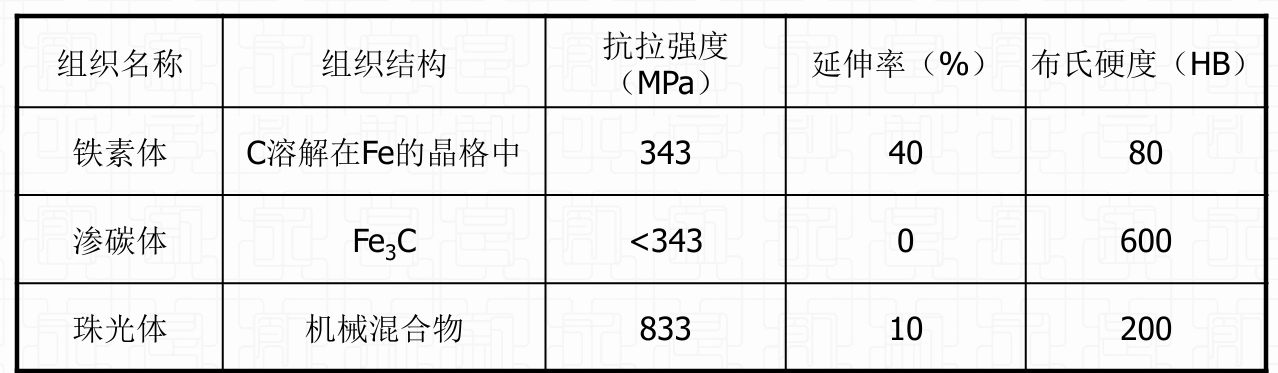
\includegraphics[width=0.7\linewidth]{../figure/santi.png} % Ensure the file exists at this path
	\caption{铁素体、渗碳体、珠光体的显微组织}
\end{figure}

\begin{figure}[H]
	\centering
	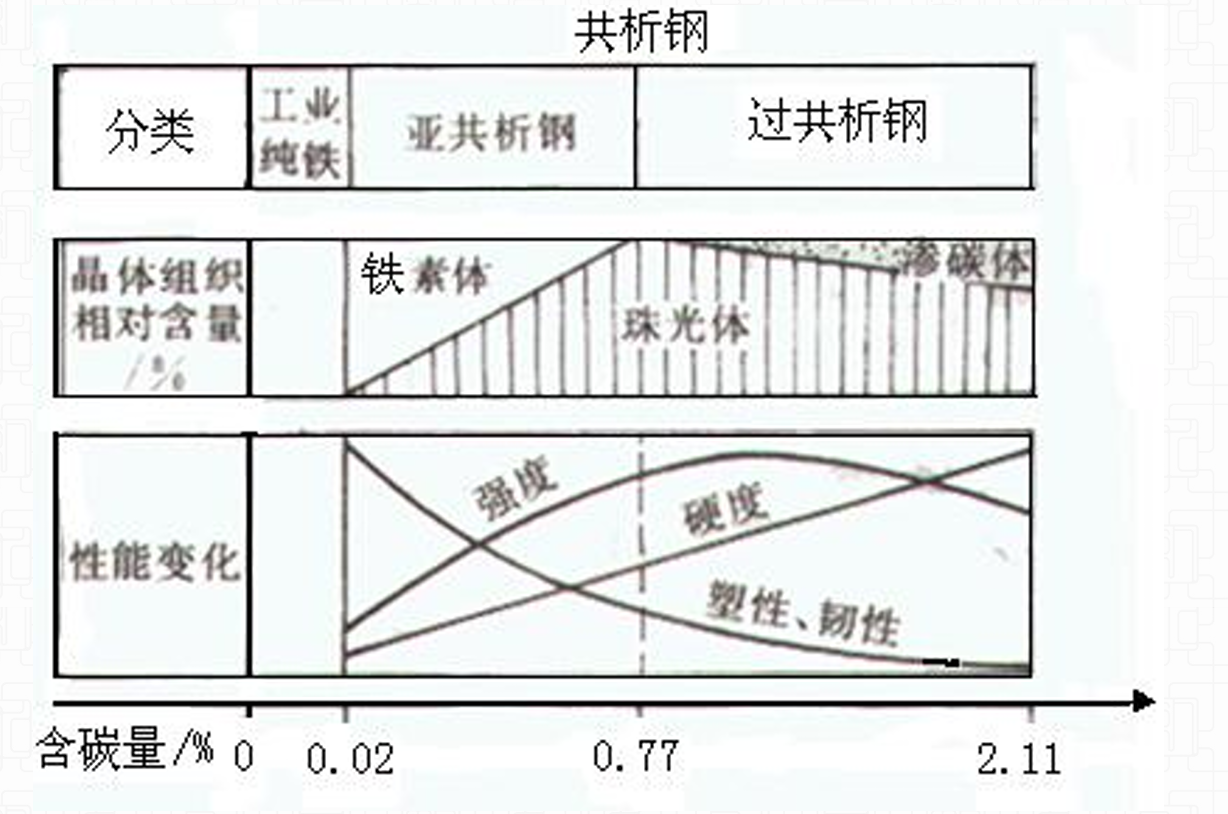
\includegraphics[width=0.7\linewidth]{../figure/qiangdubianhua.png} % Ensure the file exists at this path
	\caption{强度先上升后下降}
\end{figure}

\begin{description}

  \item[弹性阶段(OA段)]
    在 OA 阶段,如果卸去荷载,试件将恢复原状,表现为弹性变形。与 A 点相对应的应力称为\emph{弹性极限}。此阶段应力与应变成正比,即
    \[
      \sigma = E \,\varepsilon
    \]
    其中 $E$ 为弹性模量。

  \item[屈服阶段(AB段)]
    图中 B 点是此阶段应力最高点,称为\emph{屈服上限}。由于 B 点稳定易测,以其应力值作为材料抗力指标,称为\emph{屈服强度},记作 $\sigma_s$。钢材受力达 $\sigma_s$ 后,将迅速产生大量塑性变形,虽未断裂但已丧失弹性恢复能力,因此设计中常以屈服点作为强度取值依据。

  \item[强化阶段(BC段)]
    对应最高点 C 的应力称为\emph{抗拉极限强度}($\sigma_u$)。工程上不仅要求高的屈服强度,还关注屈强比 $\displaystyle \frac{\sigma_s}{\sigma_u}$。屈强比越小,材料在超过屈服后还能维持更大的应力,安全性更高;但过小又会导致材料强度未被充分利用,造成资源浪费。

  \item[颈缩阶段(CD段)]
    达到极限强度后,试件进入颈缩阶段,截面积迅速减小,应力–应变曲线开始下降直至断裂。断后测得标距由 $L_0$ 伸长至 $L_1$,其伸长率定义为
    \[
      \delta = \frac{L_1 - L_0}{L_0} \times 100\%.
    \]

\end{description}

\begin{remark}
	为什么选择下屈服极限而不是上屈服极限作为屈服极限?

	下屈服极限根据应力应变曲线图更好测量,相比而言上屈服极限就没那么好记录。

	下屈服极限(Lower Yield Point)是钢材在屈服阶段进入稳定塑性流动后所能持续承受的最低应力;而上屈服极限(Upper Yield Point)只是屈服刚开始时的峰值,应力–应变曲线瞬时达到后很快下降到下屈服水平。
\end{remark}

\subsection*{冷加工强化}
将钢材在常温下进行冷拉、冷拔或冷轧,使其产生一定的塑性变形,强度明显提高,而塑性和韧性有所降低。这个过程称为\emph{冷加工强化}。

\subsection*{时效处理}
将经过冷拉的钢筋在常温下存放15–20天,或加热到100–200℃并保持2–3小时后,钢筋强度将进一步提高。这个过程称为\emph{时效处理},其中:
\begin{itemize}
  \item \textbf{自然时效}:在常温下存放15–20天;
  \item \textbf{人工时效}:加热到100–200℃并保持2–3小时。
\end{itemize}
通常对强度较低的钢筋采用自然时效,对强度较高的钢筋则需采用人工时效。

\begin{theorem}
	钢材经冷加工产生塑性变形后,塑性变形区域内的晶粒产生相对滑移,导致滑移
面下的晶粒破碎,品格歪扭畸变,滑移面变很凹凸不平,对晶粒进一步滑移起阻碍作用,
亦即提高了抵抗外力的能力,故屈服强度得以提高, 抗拉强度基本不变。同时,冷加工
强化后的钢材,由于塑性变形后滑移面减少,从而使其塑性降低,脆性增大,且变形中
产生的内应力,使钢的弹性模量降低。
\end{theorem}

碳素结构钢材牌号:屈服强度字母Q、屈服强度数值、质量等级符
号(ABCD,从坏到好),脱氧方法符号(F、Z、TZ)

优质碳素结构钢的性质主要取决于含碳量。含碳量高则强度、硬度高,塑性、
韧性低。

\section{钢材腐蚀与预防}

\begin{definition}
	钢材表面与周围介质发生作用而引起破坏的现象称作腐蚀(锈蚀),腐蚀可分为化学腐蚀和电化学腐蚀。
\end{definition}

\paragraph{化学腐蚀}

化学腐蚀是指钢材表面与周围介质发生化学反应而引起的破坏。其特点是腐蚀速率较慢。

\paragraph{电化学腐蚀}

电化学腐蚀是指钢材表面与周围介质发生电化学反应而引起的破坏。其特点是腐蚀速率较快。

\begin{theorem}
	预防方法有:
	\begin{enumerate}
		\item 采用耐候钢,耐候钢即耐大气腐蚀钢。耐候钢是在碳素钢和低合金钢中加入少量铜、铬
、镍、钼等合金元素而制成。
		\item 用耐腐蚀性好的金属,以电镀或喷镀的方法覆盖在钢材表面,提高钢材的
耐腐蚀能力。分为阴极覆盖和阳极覆盖,阳极覆盖时,被保护金属起到正极还原的效果,阴极覆盖相反,所以阴极覆盖的保护膜破碎后会起到加速腐蚀的效果。
		\item 在钢材表面用非金属材料作为保护膜,与环境介质隔离,以避免或减缓
腐蚀。如喷涂涂料、搪瓷和塑料等。
	\end{enumerate}
\end{theorem}

\begin{remark}
	在正常的混凝土中pH值约为12,这时在钢材表面能形成碱性氧化膜(钝化
膜),对钢筋起保护作用。若混凝土碳化后,由于碱度降低(中性化)会失去
对钢筋的保护作用。此外,混凝土中氯离子达到一定浓度,也会严重破坏表面
的钝化膜。
\end{remark}

\begin{example}
  东北地区公路桥用了20年后发生混凝土钢筋腐蚀,试分析原因。
  \begin{enumerate}
    \item 钢筋用量中含有有害物质:
  \begin{itemize}
    \item 氯离子(Cl$^-$):氯离子会破坏钢筋表面的氧化膜,与 Fe$^{3+}$ 生成可溶性的氯铁配合物,破坏钝化膜,导致钢筋被侵蚀。
    \item 硫酸根离子(SO$_4^{2-}$):硫酸盐会与铝酸三钙反应生成钙矾石,导致体积膨胀,进而引起混凝土开裂,促进腐蚀。
  \end{itemize}
  \item 东北冬天气候寒冷,冬春季气温变化幅度大,存在冻土。多年冻融反复作用,导致混凝土内部产生裂缝,进而加速钢筋的腐蚀。
  \item   东北地区水分含量较高,水分渗透到钢筋表面,形成电解质溶液,促进电化学腐蚀。
  \item   二氧化碳渗透引起混凝土碳化,降低碱性,破坏钢筋的钝化保护层,易发生锈蚀。
  \item 施工后养护时间短或方法不当,后期缺少维护,混凝土强度和致密性不足。
  \end{enumerate}
  
\end{example}

\begin{example}
  为什么海砂和海水不能用于钢筋混凝土?

海砂和海水中含有大量的氯化钠(NaCl),会释放出氯离子(Cl$^-$)。这些氯离子能够穿透混凝土保护层,到达钢筋表面(具体表现为和 Fe$^{3+}$ 生成可溶性的氯铁配合物),破坏钢筋表面形成的致密氧化膜,导致钢筋发生腐蚀。
\end{example}

\ifx\allfiles\undefined
\end{document}
\fi